%
% This is the LaTeX template file for lecture notes for CS294-8,
% Computational Biology for Computer Scientists.  When preparing 
% LaTeX notes for this class, please use this template.
%
% To familiarize yourself with this template, the body contains
% some examples of its use.  Look them over.  Then you can
% run LaTeX on this file.  After you have LaTeXed this file then
% you can look over the result either by printing it out with
% dvips or using xdvi.
%
% This template is based on the template for Prof. Sinclair's CS 270.

\documentclass[twoside]{article}
\usepackage{graphics}
\usepackage{amsfonts}
\usepackage{amsmath}
\usepackage{tikz}



\usetikzlibrary{chains,fit,shapes}
\setlength{\oddsidemargin}{0.25 in}
\setlength{\evensidemargin}{-0.25 in}
\setlength{\topmargin}{-0.6 in}
\setlength{\textwidth}{6.5 in}
\setlength{\textheight}{8.5 in}
\setlength{\headsep}{0.75 in}
\setlength{\parindent}{0 in}
\setlength{\parskip}{0.1 in}

%
% The following commands set up the lecnum (lecture number)
% counter and make various numbering schemes work relative
% to the lecture number.
%
\newcounter{lecnum}
\renewcommand{\thepage}{\thelecnum-\arabic{page}}
\renewcommand{\thesection}{\thelecnum.\arabic{section}}
\renewcommand{\theequation}{\thelecnum.\arabic{equation}}
\renewcommand{\thefigure}{\thelecnum.\arabic{figure}}
\renewcommand{\thetable}{\thelecnum.\arabic{table}}

%
% The following macro is used to generate the header.
%
\newcommand{\chno}[4]{
   \pagestyle{headings}
   \thispagestyle{plain}
   \newpage
   \setcounter{lecnum}{#1}
   \setcounter{page}{1}
   \noindent
   \begin{center}
   \framebox{
      \vbox{\vspace{2mm}
    \hbox to 6.28in { {\bf CIS 511: Theory of Computation
                        \hfill Jan 19, 2017} }
       \vspace{4mm}
       \hbox to 6.28in { {\Large \hfill Lecture #1: #2  \hfill} }
       \vspace{2mm}
       \hbox to 6.28in { {\it Professor #3 \hfill #4} }
      \vspace{2mm}}
   }
   \end{center}
   \markboth{Lecture #1: #2}{Lecture #1: #2}
   {\bf NB}: {\it These notes are from CIS511 at Penn. The course followed Michael Sipser's \textit{Introduction to the Theory of Computation (3ed)} text.}
   \vspace*{4mm}
}

%
% Convention for citations is authors' initials followed by the year.
% For example, to cite a paper by Leighton and Maggs you would type
% \cite{LM89}, and to cite a paper by Strassen you would type \cite{S69}.
% (To avoid bibliography problems, for now we redefine the \cite command.)
% Also commands that create a suitable format for the reference list.
\renewcommand{\cite}[1]{[#1]}
\def\beginrefs{\begin{list}%
        {[\arabic{equation}]}{\usecounter{equation}
         \setlength{\leftmargin}{2.0truecm}\setlength{\labelsep}{0.4truecm}%
         \setlength{\labelwidth}{1.6truecm}}}
\def\endrefs{\end{list}}
\def\bibentry#1{\item[\hbox{[#1]}]}

%Use this command for a figure; it puts a figure in wherever you want it.
%usage: \fig{NUMBER}{SPACE-IN-INCHES}{CAPTION}
\newcommand{\fig}[3]{
			\vspace{#2}
			\begin{center}
			Figure \thelecnum.#1:~#3
			\end{center}
	}
% Use these for theorems, lemmas, proofs, etc.
\newtheorem{theorem}{Theorem}[lecnum]
\newtheorem{lemma}[theorem]{Lemma}
\newtheorem{proposition}[theorem]{Proposition}
\newtheorem{claim}[theorem]{Claim}
\newtheorem{corollary}[theorem]{Corollary}
\newtheorem{definition}[theorem]{Definition}
\newenvironment{proof}{{\bf Proof:}}{\hfill\rule{2mm}{2mm}}

% **** IF YOU WANT TO DEFINE ADDITIONAL MACROS FOR YOURSELF, PUT THEM HERE:

\begin{document}
%FILL IN THE RIGHT INFO.
%\lecture{**LECTURE-NUMBER**}{**DATE**}{**LECTURER**}{**SCRIBE**}
\chno{3}{Regular Language Wrap-up and Intro to Turing Machines}{Sampath Kannan}{Zach Schutzman}
%\footnotetext{These notes are partially based on those of Nigel Mansell.}

% **** YOUR NOTES GO HERE:

% Some general latex examples and examples making use of the
% macros follow.  
%**** IN GENERAL, BE BRIEF. LONG SCRIBE NOTES, NO MATTER HOW WELL WRITTEN,
%**** ARE NEVER READ BY ANYBODY.


\section*{The rest of Regular Languages}

Recall, regular languages are those recognized by DFAs, NFAs, and described by regular expressions

Are there languages that are not regular?  Trivially, yes.  The set of all languages is uncountable, but the set of all regular languages is countable.

How can we determine that a language is \textit{not} regular?





\theorem{\textbf{The Pumping Lemma} (for regular languages): If $L$ is a regular language, then there exists a constant $p$, called its $\textbf{pumping length}$, such that if $x\in L$ and $|x|\geq p$, then $x$ can be written as $x=uvw$, where $v$ is non-empty, $|uv|\leq p$, and $uv^iw\in L$ for any $i \in \mathbb{N}$.}

\begin{proof}
	Suppose $L$ is regular.  Then there exists a DFA $M$ that recognizes $L$.  Say $M$ has $p$ states ($|Q|=p$).  Suppose $L$ contains some string $x$, $|x| > p$.  Then by the Pigeonhole Principle, the path of $x$ must pass through at least one state at least twice.  Equivalently, the path of $x$ contains some cycle.  
	
	Let's think of $x$ as broken into 3 parts: $uvw$, where $u$ is the portion before the cycle, $v$ is the cycle, and $w$ is the portion after the cycle.  We will allow $u$ or $w$ to be empty, but $v$ must be non-empty.  Note that $x\in L $ implies $ uw \in L$, and more generally that $uv^iw\in L$, for any $i\in \mathbb{N}$.  
	
	We also note that $|uv|\leq p$, that is there will always be a cycle before processing $p$ characters.
	
\end{proof}

\corollary{A language is not regular if there does not exist any way to break a string of length greater than $p$ into a satisfactory $uvw$.}



\textbf{Example:} \claim{The language $L=\{0^n 1^n | n\in \mathbb{N}  \}$ is not regular.}

\begin{proof}
	
	Suppose, for the sake of contradiction, that $L$ is regular with pumping length $p$.  Consider the string $0^p 1^p$. Since we have $|uv| \leq p$, $v$ is of the form $0^k$, for some $1\leq k\leq p$.  The Pumping lemma asserts that $uv^iw$ is in $L$ for all $i\in \mathbb{N}$.  But the string $uv^2w$ has more $0$s than $1$s, and is not in $L$.  This is a contradiction, therefore $L$ is not a regular language.
	
	
\end{proof}






\textbf{Example:} \claim{The language $L=\{x\# y | |x| = |y|  \}$ is not regular.}

\begin{proof}
	
	The class of regular languages is closed under intersection.  Suppose, for the sake of contradiction, that $L$ is regular.  Let the language $K = \{ 0^* \# 1^*\}$.  $K$ is regular, as it is recognized by the following machine:\\
	

\begin{center}
	\begin{tikzpicture}[scale=0.2]
	\tikzstyle{every node}+=[inner sep=0pt]
	\draw [black] (12.8,-24) circle (3);
	\draw [black] (31.6,-24.2) circle (3);
	\draw [black] (31.6,-24.2) circle (2.4);
	\draw [black] (21.8,-34.4) circle (3);
	\draw [black] (6.2,-24) -- (9.8,-24);
	\fill [black] (9.8,-24) -- (9,-23.5) -- (9,-24.5);
	\draw [black] (15.8,-24.03) -- (28.6,-24.17);
	\fill [black] (28.6,-24.17) -- (27.81,-23.66) -- (27.79,-24.66);
	\draw (22.2,-24.61) node [below] {$\#$};
	\draw [black] (12.503,-21.027) arc (213.44395:-74.55605:2.25);
	\draw (16.11,-17.16) node [above] {$0$};
	\fill [black] (14.98,-21.96) -- (15.92,-21.93) -- (15.37,-21.1);
	\draw [black] (14.76,-26.27) -- (19.84,-32.13);
	\fill [black] (19.84,-32.13) -- (19.69,-31.2) -- (18.94,-31.85);
	\draw (16.75,-30.65) node [left] {$1$};
	\draw [black] (31.41,-21.218) arc (211.38014:-76.61986:2.25);
	\draw (35.16,-17.45) node [above] {$1$};
	\fill [black] (33.85,-22.24) -- (34.79,-22.25) -- (34.27,-21.39);
	\draw [black] (29.52,-26.36) -- (23.88,-32.24);
	\fill [black] (23.88,-32.24) -- (24.79,-32.01) -- (24.07,-31.31);
	\draw (26.17,-27.83) node [left] {$0$};
	\draw [black] (24.507,-35.666) arc (92.65981:-195.34019:2.25);
	\draw (27.77,-40.17) node [below] {$0,1$};
	\fill [black] (22.44,-37.32) -- (21.98,-38.14) -- (22.98,-38.09);
	\end{tikzpicture}
\end{center}

	
	Let's consider $K\cap L$.  This language is $K\cap L = \{0^n \# 1^n | n\in\mathbb{N}\}$.  By a slight adjustment to the previous proof, we can say that $K\cap L$ is not regular.  This contradicts the assumption that both $K$ and $L$ are regular, and since we know that $K$ is regular, it must be the case that $L$ is not.
	
	
\end{proof}

\corollary{\textbf{DFAs can't count!}}



\section*{Turing Machines}

We are moving from the simplest model of computation to the 'most'.  We can think of a DFA as receiving an input on a tape, reading one character at a time, and only moving forward, and changing states according to the currently read character and the current state, via $\delta$.

We can identify three principal limitations:

\begin{enumerate}
	\item The head doesn't pass the end of the tape
	\item The tape is read-only
	\item The head only moves forward
\end{enumerate}


For a Turing machine, we lift all three of these limitations.  The head can move left and right, it can read and write, and it can move beyond the input.

We are going to expand the tape alphabet $\Gamma$ to be a proper superset of $\Sigma$, and also containing a blank symbol $\sqcup$.

\claim{Our language $L = \{0^n \# 1^n | n\in \mathbb{N}\}$ can be recognized by a Turing Machine.}

\begin{proof}
	
	
	Consider an example input below.  First, we can scan the string to validate it is of the correct form, if not, reject.  Assume that it is.
	\begin{center}
		

	\begin{tikzpicture}
	\tikzstyle{every path}=[very thick]
	
	\edef\sizetape{0.7cm}
	\tikzstyle{tmtape}=[draw,minimum size=\sizetape]
	\tikzstyle{tmhead}=[arrow box,draw,minimum size=.5cm,arrow box
	arrows={east:.25cm, west:0.25cm}]
	
	%% Draw TM tape
	\begin{scope}[start chain=1 going right,node distance=-0.15mm]

	\node [on chain=1,tmtape] (input) {0};
	\node [on chain=1,tmtape] {0};
	\node [on chain=1,tmtape] {\dots};
	\node [on chain=1,tmtape] {\#};

	
	
	
	\node [on chain=1,tmtape] {1};
	\node [on chain=1,tmtape] {\dots};

		\node [on chain=1,tmtape] {1};

	\node [on chain=1,tmtape] {$\sqcup$};
	\node [on chain=1,tmtape] {$\sqcup$};
		\node [on chain=1,tmtape] {\dots};
			\node [on chain=1,tmtape,draw=none] {$\ldots$};

	\end{scope}
	
	\end{tikzpicture}
	
		\end{center}
	
	The following algorithm determines if the string is in $L$:
	
	\begin{enumerate}
		\item[] Replace the first zero on the tape with a special marker symbol.
		\item[] Traverse the tape and replace the first one with a marker symbol.
		\item[] Repeat until you either run out of zeros or ones.
		
	
		
		\item[] If all symbols are marked, accept, otherwise, reject.
	\end{enumerate}
	

\end{proof}



\definition{A \textbf{Turing Machine} is a 7-tuple $(Q,q_0,\Sigma,\Gamma,\delta,q_a, q_r)$.}

\begin{enumerate}
	\item[] $Q$ is the set of states
	\item[] $q_0$ is the start state
	\item[] $\Sigma$ is the input alphabet
	\item[] $\Gamma$ is the tape alphabet, a proper superset of $\Sigma$
	\item[] $\delta: Q\times\Gamma\rightarrow Q\times\Gamma\times\{L,R\}$ is the transition function.
	\item[] $q_a$ is the accept state
	\item[] $q_r$ is the reject state.
	
\end{enumerate}

The transition function maps the current state and the currently read character to the next state, the character to write on that cell, and a LEFT or RIGHT move.  The machine halts when it reaches $q_a$ or $q_r$, by definition.

\definition{Given a Turing machine $M$, the language \textbf{recognized} by $M$ is the set of all strings that cause $M$ to move to $q_a$.}

If $M$ recognizes $L$ and $x\notin L$, there are two possibilities:

\begin{enumerate}
	\item $M$ reaches $q_r$
	\item $M$ computes infinitely and never reaches $q_a$ or $q_r$.  That is, $M$ 'loops forever'.
\end{enumerate}

In both of these cases, we say that $M$ doesn't recognize $x$, but in the second case, how do we know if $M$ really won't halt on $x$, rather than just taking a really long time?

\definition{A Turing machine $M$ \textbf{decides} a language $L$ if for all $x\in L$, $M$ reaches $q_a$ and for all $x\notin L$, $M$ reaches $q_r$.  The set of Turing decidable languages is a subset of the Turing recognizable languages.}


\definition{The \textbf{current configuration} of a Turing machine $M$ is the current state, the tape contents, and the head position at some point in time.}

The notation for this is:\\
	\begin{center}
		
		
		\begin{tikzpicture}
		\tikzstyle{every path}=[very thick]
		
		\edef\sizetape{0.7cm}
		\tikzstyle{tmtape}=[draw,minimum size=\sizetape]
		\tikzstyle{tmhead}=[arrow box,draw,minimum size=.5cm,arrow box
		arrows={east:.25cm, west:0.25cm}]
		
		%% Draw TM tape
		\begin{scope}[start chain=1 going right,node distance=-0.15mm]
		
		\node [on chain=1,tmtape] (input) {};
		\node [on chain=1,tmtape] {};
		\node [on chain=1,tmtape] {};
		\node [on chain=1,tmtape] {$q_c$};
		
				
		\node [on chain=1,tmtape] {a};
		\node [on chain=1,tmtape] {\dots};
		
		\node [on chain=1,tmtape] {};
		
		\node [on chain=1,tmtape] {};
		\node [on chain=1,tmtape] {};
		\node [on chain=1,tmtape] {};
		\node [on chain=1,tmtape,draw=none] {$\ldots$};
		
		\end{scope}
		
		\end{tikzpicture}
		
	\end{center}

to denote that we are in state $q_c$ and the head is over $a$.


\textbf{Example:} Let's construct a Turing machine to recognize the language of palindromes, $L=\{w \# w^R| w = (w^R)^R\}$.




\end{document}







